\documentclass[]{article}
\usepackage{lmodern}
\usepackage{amssymb,amsmath}
\usepackage{ifxetex,ifluatex}
\usepackage{fixltx2e} % provides \textsubscript
\ifnum 0\ifxetex 1\fi\ifluatex 1\fi=0 % if pdftex
  \usepackage[T1]{fontenc}
  \usepackage[utf8]{inputenc}
\else % if luatex or xelatex
  \ifxetex
    \usepackage{mathspec}
  \else
    \usepackage{fontspec}
  \fi
  \defaultfontfeatures{Ligatures=TeX,Scale=MatchLowercase}
\fi
% use upquote if available, for straight quotes in verbatim environments
\IfFileExists{upquote.sty}{\usepackage{upquote}}{}
% use microtype if available
\IfFileExists{microtype.sty}{%
\usepackage{microtype}
\UseMicrotypeSet[protrusion]{basicmath} % disable protrusion for tt fonts
}{}
\usepackage[margin=1in]{geometry}
\usepackage{hyperref}
\hypersetup{unicode=true,
            pdftitle={ANOVA pedagogica \textasciitilde{} area.de.conhecimento},
            pdfauthor={Geiser C. Challco geiser@usp.br},
            pdfborder={0 0 0},
            breaklinks=true}
\urlstyle{same}  % don't use monospace font for urls
\usepackage{color}
\usepackage{fancyvrb}
\newcommand{\VerbBar}{|}
\newcommand{\VERB}{\Verb[commandchars=\\\{\}]}
\DefineVerbatimEnvironment{Highlighting}{Verbatim}{commandchars=\\\{\}}
% Add ',fontsize=\small' for more characters per line
\usepackage{framed}
\definecolor{shadecolor}{RGB}{248,248,248}
\newenvironment{Shaded}{\begin{snugshade}}{\end{snugshade}}
\newcommand{\AlertTok}[1]{\textcolor[rgb]{0.94,0.16,0.16}{#1}}
\newcommand{\AnnotationTok}[1]{\textcolor[rgb]{0.56,0.35,0.01}{\textbf{\textit{#1}}}}
\newcommand{\AttributeTok}[1]{\textcolor[rgb]{0.77,0.63,0.00}{#1}}
\newcommand{\BaseNTok}[1]{\textcolor[rgb]{0.00,0.00,0.81}{#1}}
\newcommand{\BuiltInTok}[1]{#1}
\newcommand{\CharTok}[1]{\textcolor[rgb]{0.31,0.60,0.02}{#1}}
\newcommand{\CommentTok}[1]{\textcolor[rgb]{0.56,0.35,0.01}{\textit{#1}}}
\newcommand{\CommentVarTok}[1]{\textcolor[rgb]{0.56,0.35,0.01}{\textbf{\textit{#1}}}}
\newcommand{\ConstantTok}[1]{\textcolor[rgb]{0.00,0.00,0.00}{#1}}
\newcommand{\ControlFlowTok}[1]{\textcolor[rgb]{0.13,0.29,0.53}{\textbf{#1}}}
\newcommand{\DataTypeTok}[1]{\textcolor[rgb]{0.13,0.29,0.53}{#1}}
\newcommand{\DecValTok}[1]{\textcolor[rgb]{0.00,0.00,0.81}{#1}}
\newcommand{\DocumentationTok}[1]{\textcolor[rgb]{0.56,0.35,0.01}{\textbf{\textit{#1}}}}
\newcommand{\ErrorTok}[1]{\textcolor[rgb]{0.64,0.00,0.00}{\textbf{#1}}}
\newcommand{\ExtensionTok}[1]{#1}
\newcommand{\FloatTok}[1]{\textcolor[rgb]{0.00,0.00,0.81}{#1}}
\newcommand{\FunctionTok}[1]{\textcolor[rgb]{0.00,0.00,0.00}{#1}}
\newcommand{\ImportTok}[1]{#1}
\newcommand{\InformationTok}[1]{\textcolor[rgb]{0.56,0.35,0.01}{\textbf{\textit{#1}}}}
\newcommand{\KeywordTok}[1]{\textcolor[rgb]{0.13,0.29,0.53}{\textbf{#1}}}
\newcommand{\NormalTok}[1]{#1}
\newcommand{\OperatorTok}[1]{\textcolor[rgb]{0.81,0.36,0.00}{\textbf{#1}}}
\newcommand{\OtherTok}[1]{\textcolor[rgb]{0.56,0.35,0.01}{#1}}
\newcommand{\PreprocessorTok}[1]{\textcolor[rgb]{0.56,0.35,0.01}{\textit{#1}}}
\newcommand{\RegionMarkerTok}[1]{#1}
\newcommand{\SpecialCharTok}[1]{\textcolor[rgb]{0.00,0.00,0.00}{#1}}
\newcommand{\SpecialStringTok}[1]{\textcolor[rgb]{0.31,0.60,0.02}{#1}}
\newcommand{\StringTok}[1]{\textcolor[rgb]{0.31,0.60,0.02}{#1}}
\newcommand{\VariableTok}[1]{\textcolor[rgb]{0.00,0.00,0.00}{#1}}
\newcommand{\VerbatimStringTok}[1]{\textcolor[rgb]{0.31,0.60,0.02}{#1}}
\newcommand{\WarningTok}[1]{\textcolor[rgb]{0.56,0.35,0.01}{\textbf{\textit{#1}}}}
\usepackage{longtable,booktabs}
\usepackage{graphicx,grffile}
\makeatletter
\def\maxwidth{\ifdim\Gin@nat@width>\linewidth\linewidth\else\Gin@nat@width\fi}
\def\maxheight{\ifdim\Gin@nat@height>\textheight\textheight\else\Gin@nat@height\fi}
\makeatother
% Scale images if necessary, so that they will not overflow the page
% margins by default, and it is still possible to overwrite the defaults
% using explicit options in \includegraphics[width, height, ...]{}
\setkeys{Gin}{width=\maxwidth,height=\maxheight,keepaspectratio}
\IfFileExists{parskip.sty}{%
\usepackage{parskip}
}{% else
\setlength{\parindent}{0pt}
\setlength{\parskip}{6pt plus 2pt minus 1pt}
}
\setlength{\emergencystretch}{3em}  % prevent overfull lines
\providecommand{\tightlist}{%
  \setlength{\itemsep}{0pt}\setlength{\parskip}{0pt}}
\setcounter{secnumdepth}{0}
% Redefines (sub)paragraphs to behave more like sections
\ifx\paragraph\undefined\else
\let\oldparagraph\paragraph
\renewcommand{\paragraph}[1]{\oldparagraph{#1}\mbox{}}
\fi
\ifx\subparagraph\undefined\else
\let\oldsubparagraph\subparagraph
\renewcommand{\subparagraph}[1]{\oldsubparagraph{#1}\mbox{}}
\fi

%%% Use protect on footnotes to avoid problems with footnotes in titles
\let\rmarkdownfootnote\footnote%
\def\footnote{\protect\rmarkdownfootnote}

%%% Change title format to be more compact
\usepackage{titling}

% Create subtitle command for use in maketitle
\providecommand{\subtitle}[1]{
  \posttitle{
    \begin{center}\large#1\end{center}
    }
}

\setlength{\droptitle}{-2em}

  \title{ANOVA \texttt{pedagogica} \textasciitilde{}
\texttt{area.de.conhecimento}}
    \pretitle{\vspace{\droptitle}\centering\huge}
  \posttitle{\par}
    \author{Geiser C. Challco \href{mailto:geiser@usp.br}{\nolinkurl{geiser@usp.br}}}
    \preauthor{\centering\large\emph}
  \postauthor{\par}
    \date{}
    \predate{}\postdate{}
  

\begin{document}
\maketitle

\begin{itemize}
\tightlist
\item
  Report as Word format: \url{factorialAnova.docx}
\item
  Report as LaTex format: \url{factorialAnova.tex}
\end{itemize}

\hypertarget{initial-data-and-preprocessing}{%
\subsection{Initial Data and
Preprocessing}\label{initial-data-and-preprocessing}}

R script: \url{factorialAnova.R} Inital data: \url{data.csv}

\hypertarget{visualization-of-data-distribution}{%
\subsubsection{Visualization of data
distribution}\label{visualization-of-data-distribution}}

\begin{Shaded}
\begin{Highlighting}[]
\KeywordTok{ggdensity}\NormalTok{(dat, }\DataTypeTok{x =} \StringTok{"pedagogica"}\NormalTok{, }\DataTypeTok{fill =} \StringTok{"lightgray"}\NormalTok{, }\DataTypeTok{title=} \StringTok{"Density of pedagogica before transformation"}\NormalTok{) }\OperatorTok{+}
\StringTok{ }\KeywordTok{stat_overlay_normal_density}\NormalTok{(}\DataTypeTok{color =} \StringTok{"red"}\NormalTok{, }\DataTypeTok{linetype =} \StringTok{"dashed"}\NormalTok{)}
\end{Highlighting}
\end{Shaded}

\includegraphics{factorialAnova_files/figure-latex/unnamed-chunk-1-1.pdf}

\hypertarget{dealing-with-positive-greater-skewness-in-pedagogica}{%
\subsubsection{Dealing with positive greater skewness in
pedagogica}\label{dealing-with-positive-greater-skewness-in-pedagogica}}

\begin{Shaded}
\begin{Highlighting}[]
\NormalTok{dat[[}\StringTok{"pedagogica"}\NormalTok{]] <-}\StringTok{ }\KeywordTok{log10}\NormalTok{(dat[[}\StringTok{"pedagogica"}\NormalTok{]])}
\end{Highlighting}
\end{Shaded}

\begin{Shaded}
\begin{Highlighting}[]
\KeywordTok{ggdensity}\NormalTok{(dat, }\DataTypeTok{x =} \StringTok{"pedagogica"}\NormalTok{, }\DataTypeTok{fill =} \StringTok{"lightgray"}\NormalTok{, }\DataTypeTok{title=} \StringTok{"Density of pedagogica after transformation"}\NormalTok{) }\OperatorTok{+}
\StringTok{ }\KeywordTok{stat_overlay_normal_density}\NormalTok{(}\DataTypeTok{color =} \StringTok{"red"}\NormalTok{, }\DataTypeTok{linetype =} \StringTok{"dashed"}\NormalTok{)}
\end{Highlighting}
\end{Shaded}

\includegraphics{factorialAnova_files/figure-latex/unnamed-chunk-3-1.pdf}

\hypertarget{summary-statistics-of-the-initial-data}{%
\subsubsection{Summary statistics of the initial
data}\label{summary-statistics-of-the-initial-data}}

\begin{Shaded}
\begin{Highlighting}[]
\KeywordTok{get_summary_stats}\NormalTok{(}\KeywordTok{group_by}\NormalTok{(dat, }\StringTok{`}\DataTypeTok{area.de.conhecimento}\StringTok{`}\NormalTok{), }\DataTypeTok{type =}\StringTok{"common"}\NormalTok{)}
\end{Highlighting}
\end{Shaded}

\begin{verbatim}
## # A tibble: 8 x 11
##   area.de.conheci~ variable     n   min   max median   iqr  mean    sd
##   <fct>            <chr>    <dbl> <dbl> <dbl>  <dbl> <dbl> <dbl> <dbl>
## 1 Ciências Agrári~ pedagog~    28     0 0.628  0.243 0.242 0.264 0.184
## 2 Ciências Biológ~ pedagog~    22     0 0.574  0.176 0.301 0.211 0.192
## 3 Ciências da Saú~ pedagog~    65     0 0.699  0.243 0.301 0.257 0.18 
## 4 Ciências Exatas~ pedagog~    48     0 0.653  0.301 0.263 0.318 0.172
## 5 Ciências Humanas pedagog~    45     0 0.699  0.352 0.336 0.329 0.197
## 6 Ciências Sociai~ pedagog~    53     0 0.653  0.301 0.336 0.322 0.199
## 7 Engenharias      pedagog~    31     0 0.628  0.301 0.155 0.297 0.163
## 8 Linguística/Let~ pedagog~    32     0 0.677  0.398 0.271 0.338 0.201
## # ... with 2 more variables: se <dbl>, ci <dbl>
\end{verbatim}

\hypertarget{check-assumptions}{%
\subsection{Check Assumptions}\label{check-assumptions}}

\hypertarget{identifying-outliers}{%
\subsubsection{Identifying outliers}\label{identifying-outliers}}

Outliers tend to increase type-I error probability, and they decrease
the calculated F statistic in ANOVA resulting in a lower chance of
reject the null hypothesis.

\begin{itemize}
\tightlist
\item
  Identified outliers using rstatix
\end{itemize}

\begin{Shaded}
\begin{Highlighting}[]
\KeywordTok{identify_outliers}\NormalTok{(}\KeywordTok{group_by}\NormalTok{(dat, }\StringTok{`}\DataTypeTok{area.de.conhecimento}\StringTok{`}\NormalTok{), }\StringTok{`}\DataTypeTok{pedagogica}\StringTok{`}\NormalTok{)}
\end{Highlighting}
\end{Shaded}

\begin{verbatim}
## # A tibble: 3 x 5
##   area.de.conhecimento ID     pedagogica is.outlier is.extreme
##   <fct>                <fct>       <dbl> <lgl>      <lgl>     
## 1 Engenharias          Obs50           0 TRUE       FALSE     
## 2 Engenharias          Obs141          0 TRUE       FALSE     
## 3 Engenharias          Obs286          0 TRUE       FALSE
\end{verbatim}

\begin{itemize}
\tightlist
\item
  Identified outliers through Boxplots
\end{itemize}

\begin{Shaded}
\begin{Highlighting}[]
\KeywordTok{Boxplot}\NormalTok{(}\StringTok{`}\DataTypeTok{pedagogica}\StringTok{`} \OperatorTok{~}\StringTok{ `}\DataTypeTok{area.de.conhecimento}\StringTok{`}\NormalTok{, }\DataTypeTok{data =}\NormalTok{ dat, }\DataTypeTok{id =} \KeywordTok{list}\NormalTok{(}\DataTypeTok{n =} \OtherTok{Inf}\NormalTok{))}
\end{Highlighting}
\end{Shaded}

\includegraphics{factorialAnova_files/figure-latex/unnamed-chunk-6-1.pdf}

\begin{verbatim}
## [1] "Obs50"  "Obs141" "Obs286"
\end{verbatim}

\hypertarget{removing-outliers-from-the-data}{%
\subsubsection{Removing outliers from the
data}\label{removing-outliers-from-the-data}}

\begin{Shaded}
\begin{Highlighting}[]
\NormalTok{outliers <-}\StringTok{ }\KeywordTok{c}\NormalTok{(}\StringTok{"Obs50"}\NormalTok{,}\StringTok{"Obs141"}\NormalTok{,}\StringTok{"Obs286"}\NormalTok{)}
\NormalTok{rdat <-}\StringTok{ }\NormalTok{dat[}\OperatorTok{!}\NormalTok{dat[[}\StringTok{"ID"}\NormalTok{]] }\OperatorTok\StringTok{ }\NormalTok{outliers,]   }\CommentTok{# table without outliers}
\end{Highlighting}
\end{Shaded}

\begin{longtable}[]{@{}lllr@{}}
\caption{Outliers table}\tabularnewline
\toprule
& ID & area.de.conhecimento & pedagogica\tabularnewline
\midrule
\endfirsthead
\toprule
& ID & area.de.conhecimento & pedagogica\tabularnewline
\midrule
\endhead
Obs50 & Obs50 & Engenharias & 0\tabularnewline
Obs141 & Obs141 & Engenharias & 0\tabularnewline
Obs286 & Obs286 & Engenharias & 0\tabularnewline
\bottomrule
\end{longtable}

\hypertarget{normality-assumption}{%
\subsubsection{Normality assumption}\label{normality-assumption}}

\textbf{Observation}:

As sample sizes increase, ANOVA remains a valid test even with the
violation of normality {[}\protect\hyperlink{references}{1},
\protect\hyperlink{references}{2}{]}. According to the central limit
theorem, the sampling distribution tends to be normal if the sample is
large enough (\texttt{n\ \textgreater{}\ 30}). Therefore, we performed
ANOVA with large samples as follows:

\begin{itemize}
\item
  In cases with the sample size greater than 30
  (\texttt{n\ \textgreater{}\ 30}), we adopted a significance level of
  \texttt{p\ \textless{}\ 0.01} instead a significance level of
  \texttt{p\ \textless{}\ 0.05}.
\item
  For samples with \texttt{n\ \textgreater{}\ 50} observation, we
  adopted D'Agostino-Pearson test that offers better accuracy for larger
  samples {[}\protect\hyperlink{references}{3}{]}.
\item
  For samples' size between \texttt{n\ \textgreater{}\ 100} and
  \texttt{n\ \textless{}=\ 200}, we ignored both tests (Shapiro and
  D'Agostino-Persons), and our decision of normality were based only in
  the interpretation of QQ-plots and histograms because these tests tend
  to be too sensitive with values greater than 200
  {[}\protect\hyperlink{references}{3}{]}.
\item
  For samples with \texttt{n\ \textgreater{}\ 200} observation, we
  ignore the normality assumption based on the central theorem limit,
  and taking only into account the homogeneity assumption.
\end{itemize}

\hypertarget{checking-normality-assumption-in-the-residual-model}{%
\paragraph{Checking normality assumption in the residual
model}\label{checking-normality-assumption-in-the-residual-model}}

\begin{Shaded}
\begin{Highlighting}[]
\NormalTok{mdl <-}\StringTok{ }\KeywordTok{lm}\NormalTok{(}\StringTok{`}\DataTypeTok{pedagogica}\StringTok{`} \OperatorTok{~}\StringTok{ `}\DataTypeTok{area.de.conhecimento}\StringTok{`}\NormalTok{, }\DataTypeTok{data =}\NormalTok{ rdat)}
\KeywordTok{normality_test}\NormalTok{(}\KeywordTok{residuals}\NormalTok{(mdl))}
\end{Highlighting}
\end{Shaded}

\begin{verbatim}
##     n statistic     method            p p.signif normality
## 1 321  36.25437 D'Agostino 1.341109e-08     ****         -
\end{verbatim}

The QQ plot used to evaluate normality assumption

\begin{Shaded}
\begin{Highlighting}[]
\KeywordTok{qqPlot}\NormalTok{(}\KeywordTok{residuals}\NormalTok{(mdl))}
\end{Highlighting}
\end{Shaded}

\includegraphics{factorialAnova_files/figure-latex/unnamed-chunk-10-1.pdf}

\begin{verbatim}
## Obs322 Obs188 
##    313    182
\end{verbatim}

\hypertarget{checking-normality-assumption-for-each-group}{%
\paragraph{Checking normality assumption for each
group}\label{checking-normality-assumption-for-each-group}}

\begin{Shaded}
\begin{Highlighting}[]
\KeywordTok{normality_test_at}\NormalTok{(}\KeywordTok{group_by}\NormalTok{(rdat, }\StringTok{`}\DataTypeTok{area.de.conhecimento}\StringTok{`}\NormalTok{), }\StringTok{"pedagogica"}\NormalTok{)}
\end{Highlighting}
\end{Shaded}

\begin{verbatim}
##                  variable       area.de.conhecimento  n  statistic
## 1              pedagogica          Ciências Agrárias 28  0.9498630
## 2              pedagogica        Ciências Biológicas 22  0.8900311
## Omnibus  Test  pedagogica          Ciências da Saúde 65  3.4534213
## 11             pedagogica Ciências Exatas e da Terra 48  0.9501681
## 12             pedagogica           Ciências Humanas 45  0.9549532
## Omnibus  Test1 pedagogica Ciências Sociais Aplicadas 53 13.8151630
## 13             pedagogica                Engenharias 28  0.9577111
## 14             pedagogica Linguística/Letras e Artes 32  0.9279369
##                      method           p p.signif normality
## 1              Shapiro-Wilk 0.196565111       ns       YES
## 2              Shapiro-Wilk 0.018876425        *        NO
## Omnibus  Test    D'Agostino 0.177868523       ns       YES
## 11             Shapiro-Wilk 0.040607637       ns       YES
## 12             Shapiro-Wilk 0.078371098       ns       YES
## Omnibus  Test1   D'Agostino 0.001000174        *        NO
## 13             Shapiro-Wilk 0.307318051       ns       YES
## 14             Shapiro-Wilk 0.034319484       ns       YES
\end{verbatim}

\begin{itemize}
\tightlist
\item
  QQ plot in the \textbf{area.de.conhecimento}: ``Ciências Agrárias''
\end{itemize}

\begin{Shaded}
\begin{Highlighting}[]
\KeywordTok{qqPlot}\NormalTok{( }\OperatorTok{~}\StringTok{ `}\DataTypeTok{pedagogica}\StringTok{`}\NormalTok{, }\DataTypeTok{data =}\NormalTok{ rdat[}\KeywordTok{which}\NormalTok{(rdat[}\StringTok{"area.de.conhecimento"}\NormalTok{] }\OperatorTok{==}\StringTok{ "Ciências Agrárias"}\NormalTok{),])}
\end{Highlighting}
\end{Shaded}

\includegraphics{factorialAnova_files/figure-latex/unnamed-chunk-12-1.pdf}

\begin{verbatim}
## Obs160 Obs166 
##     14     15
\end{verbatim}

\begin{itemize}
\tightlist
\item
  QQ plot in the \textbf{area.de.conhecimento}: ``Ciências Biológicas''
\end{itemize}

\begin{Shaded}
\begin{Highlighting}[]
\KeywordTok{qqPlot}\NormalTok{( }\OperatorTok{~}\StringTok{ `}\DataTypeTok{pedagogica}\StringTok{`}\NormalTok{, }\DataTypeTok{data =}\NormalTok{ rdat[}\KeywordTok{which}\NormalTok{(rdat[}\StringTok{"area.de.conhecimento"}\NormalTok{] }\OperatorTok{==}\StringTok{ "Ciências Biológicas"),])}
\end{Highlighting}
\end{Shaded}

\includegraphics{factorialAnova_files/figure-latex/unnamed-chunk-13-1.pdf}

\begin{verbatim}
## Obs171 Obs178 
##     12     13
\end{verbatim}

\begin{itemize}
\tightlist
\item
  QQ plot in the \textbf{area.de.conhecimento}: ``Ciências da Saúde''
\end{itemize}

\begin{Shaded}
\begin{Highlighting}[]
\KeywordTok{qqPlot}\NormalTok{( }\OperatorTok{~}\StringTok{ `}\DataTypeTok{pedagogica}\StringTok{`}\NormalTok{, }\DataTypeTok{data =}\NormalTok{ rdat[}\KeywordTok{which}\NormalTok{(rdat[}\StringTok{"area.de.conhecimento"}\NormalTok{] }\OperatorTok{==}\StringTok{ "Ciências da Saúde"),])}
\end{Highlighting}
\end{Shaded}

\includegraphics{factorialAnova_files/figure-latex/unnamed-chunk-14-1.pdf}

\begin{verbatim}
## Obs322 Obs208 
##     62     36
\end{verbatim}

\begin{itemize}
\tightlist
\item
  QQ plot in the \textbf{area.de.conhecimento}: ``Ciências Exatas e da
  Terra''
\end{itemize}

\begin{Shaded}
\begin{Highlighting}[]
\KeywordTok{qqPlot}\NormalTok{( }\OperatorTok{~}\StringTok{ `}\DataTypeTok{pedagogica}\StringTok{`}\NormalTok{, }\DataTypeTok{data =}\NormalTok{ rdat[}\KeywordTok{which}\NormalTok{(rdat[}\StringTok{"area.de.conhecimento"}\NormalTok{] }\OperatorTok{==}\StringTok{ "Ciências Exatas e da Terra"}\NormalTok{),])}
\end{Highlighting}
\end{Shaded}

\includegraphics{factorialAnova_files/figure-latex/unnamed-chunk-15-1.pdf}

\begin{verbatim}
## Obs127  Obs52 
##     21      9
\end{verbatim}

\begin{itemize}
\tightlist
\item
  QQ plot in the \textbf{area.de.conhecimento}: ``Ciências Humanas''
\end{itemize}

\begin{Shaded}
\begin{Highlighting}[]
\KeywordTok{qqPlot}\NormalTok{( }\OperatorTok{~}\StringTok{ `}\DataTypeTok{pedagogica}\StringTok{`}\NormalTok{, }\DataTypeTok{data =}\NormalTok{ rdat[}\KeywordTok{which}\NormalTok{(rdat[}\StringTok{"area.de.conhecimento"}\NormalTok{] }\OperatorTok{==}\StringTok{ "Ciências Humanas"}\NormalTok{),])}
\end{Highlighting}
\end{Shaded}

\includegraphics{factorialAnova_files/figure-latex/unnamed-chunk-16-1.pdf}

\begin{verbatim}
## Obs188 Obs119 
##     33     22
\end{verbatim}

\begin{itemize}
\tightlist
\item
  QQ plot in the \textbf{area.de.conhecimento}: ``Ciências Sociais
  Aplicadas''
\end{itemize}

\begin{Shaded}
\begin{Highlighting}[]
\KeywordTok{qqPlot}\NormalTok{( }\OperatorTok{~}\StringTok{ `}\DataTypeTok{pedagogica}\StringTok{`}\NormalTok{, }\DataTypeTok{data =}\NormalTok{ rdat[}\KeywordTok{which}\NormalTok{(rdat[}\StringTok{"area.de.conhecimento"}\NormalTok{] }\OperatorTok{==}\StringTok{ "Ciências Sociais Aplicadas"}\NormalTok{),])}
\end{Highlighting}
\end{Shaded}

\includegraphics{factorialAnova_files/figure-latex/unnamed-chunk-17-1.pdf}

\begin{verbatim}
## Obs62 Obs27 
##    20    11
\end{verbatim}

\begin{itemize}
\tightlist
\item
  QQ plot in the \textbf{area.de.conhecimento}: ``Engenharias''
\end{itemize}

\begin{Shaded}
\begin{Highlighting}[]
\KeywordTok{qqPlot}\NormalTok{( }\OperatorTok{~}\StringTok{ `}\DataTypeTok{pedagogica}\StringTok{`}\NormalTok{, }\DataTypeTok{data =}\NormalTok{ rdat[}\KeywordTok{which}\NormalTok{(rdat[}\StringTok{"area.de.conhecimento"}\NormalTok{] }\OperatorTok{==}\StringTok{ "Engenharias"}\NormalTok{),])}
\end{Highlighting}
\end{Shaded}

\includegraphics{factorialAnova_files/figure-latex/unnamed-chunk-18-1.pdf}

\begin{verbatim}
##  Obs74 Obs148 
##      8     11
\end{verbatim}

\begin{itemize}
\tightlist
\item
  QQ plot in the \textbf{area.de.conhecimento}: ``Linguística/Letras e
  Artes''
\end{itemize}

\begin{Shaded}
\begin{Highlighting}[]
\KeywordTok{qqPlot}\NormalTok{( }\OperatorTok{~}\StringTok{ `}\DataTypeTok{pedagogica}\StringTok{`}\NormalTok{, }\DataTypeTok{data =}\NormalTok{ rdat[}\KeywordTok{which}\NormalTok{(rdat[}\StringTok{"area.de.conhecimento"}\NormalTok{] }\OperatorTok{==}\StringTok{ "Linguística/Letras e Artes"}\NormalTok{),])}
\end{Highlighting}
\end{Shaded}

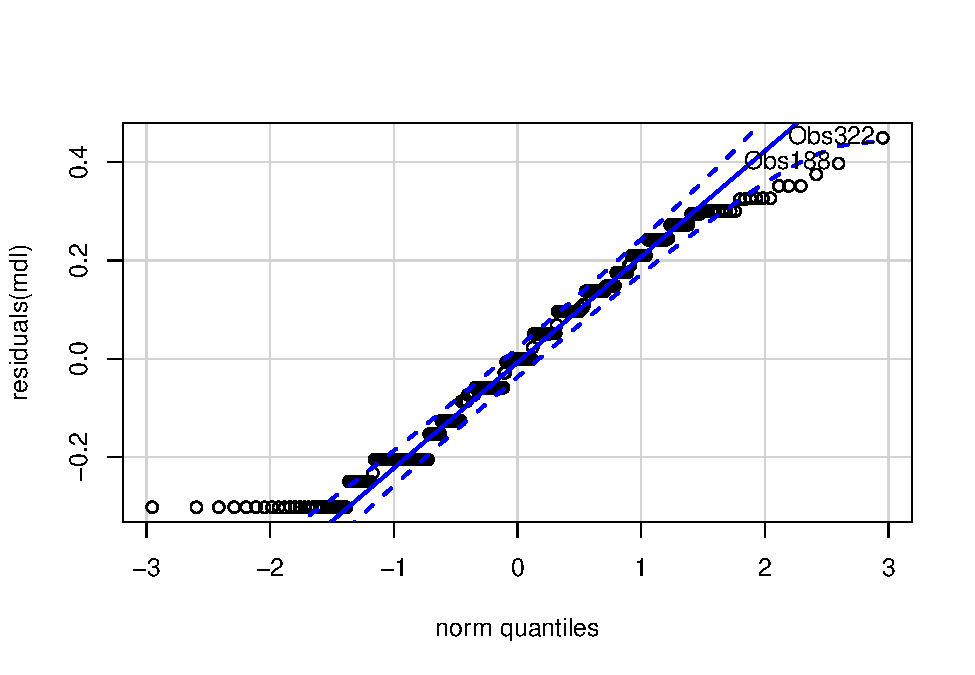
\includegraphics{factorialAnova_files/figure-latex/unnamed-chunk-19-1.pdf}

\begin{verbatim}
## Obs234  Obs18 
##     23      2
\end{verbatim}

\hypertarget{removing-data-that-affect-normality}{%
\paragraph{Removing data that affect
normality}\label{removing-data-that-affect-normality}}

\begin{Shaded}
\begin{Highlighting}[]
\NormalTok{non.normal <-}\StringTok{ }\KeywordTok{c}\NormalTok{(}\StringTok{"Obs15"}\NormalTok{,}\StringTok{"Obs27"}\NormalTok{,}\StringTok{"Obs62"}\NormalTok{,}\StringTok{"Obs110"}\NormalTok{,}\StringTok{"Obs140"}\NormalTok{,}\StringTok{"Obs178"}\NormalTok{)}
\NormalTok{sdat <-}\StringTok{ }\NormalTok{rdat[}\OperatorTok{!}\NormalTok{rdat[[}\StringTok{"ID"}\NormalTok{]] }\OperatorTok\StringTok{ }\NormalTok{non.normal,]   }\CommentTok{# table without non-normal and outliers}
\end{Highlighting}
\end{Shaded}

\begin{longtable}[]{@{}lllr@{}}
\caption{Non-normal data table}\tabularnewline
\toprule
& ID & area.de.conhecimento & pedagogica\tabularnewline
\midrule
\endfirsthead
\toprule
& ID & area.de.conhecimento & pedagogica\tabularnewline
\midrule
\endhead
Obs15 & Obs15 & Ciências Sociais Aplicadas & 0.6283889\tabularnewline
Obs27 & Obs27 & Ciências Sociais Aplicadas & 0.0000000\tabularnewline
Obs62 & Obs62 & Ciências Sociais Aplicadas & 0.6532125\tabularnewline
Obs110 & Obs110 & Ciências Sociais Aplicadas & 0.0000000\tabularnewline
Obs140 & Obs140 & Ciências Biológicas & 0.0000000\tabularnewline
Obs178 & Obs178 & Ciências Biológicas & 0.5440680\tabularnewline
\bottomrule
\end{longtable}

\hypertarget{performing-normality-test-without-data-that-affect-normality}{%
\paragraph{Performing normality test without data that affect
normality}\label{performing-normality-test-without-data-that-affect-normality}}

\begin{Shaded}
\begin{Highlighting}[]
\NormalTok{mdl <-}\StringTok{ }\KeywordTok{lm}\NormalTok{(}\StringTok{`}\DataTypeTok{pedagogica}\StringTok{`} \OperatorTok{~}\StringTok{ `}\DataTypeTok{area.de.conhecimento}\StringTok{`}\NormalTok{, }\DataTypeTok{data =}\NormalTok{ sdat)}
\KeywordTok{normality_test}\NormalTok{(}\KeywordTok{residuals}\NormalTok{(mdl))}
\end{Highlighting}
\end{Shaded}

\begin{longtable}[]{@{}rrllll@{}}
\toprule
n & statistic & method & p & p.signif & normality\tabularnewline
\midrule
\endhead
315 & 31.015 & D'Agostino & \textless{} 0.0001 & **** & -\tabularnewline
\bottomrule
\end{longtable}

\begin{Shaded}
\begin{Highlighting}[]
\KeywordTok{normality_test_at}\NormalTok{(}\KeywordTok{group_by}\NormalTok{(sdat, }\StringTok{`}\DataTypeTok{area.de.conhecimento}\StringTok{`}\NormalTok{), }\StringTok{"pedagogica"}\NormalTok{)}
\end{Highlighting}
\end{Shaded}

\begin{longtable}[]{@{}llrrllll@{}}
\toprule
variable & area.de.conhecimento & n & statistic & method & p & p.signif
& normality\tabularnewline
\midrule
\endhead
pedagogica & Ciências Agrárias & 28 & 0.9499 & Shapiro-Wilk & 0.1966 &
ns & YES\tabularnewline
pedagogica & Ciências Biológicas & 20 & 0.9071 & Shapiro-Wilk & 0.0561 &
ns & YES\tabularnewline
pedagogica & Ciências da Saúde & 65 & 3.4534 & D'Agostino & 0.1779 & ns
& YES\tabularnewline
pedagogica & Ciências Exatas e da Terra & 48 & 0.9502 & Shapiro-Wilk &
0.0406 & * & YES\tabularnewline
pedagogica & Ciências Humanas & 45 & 0.9550 & Shapiro-Wilk & 0.0784 & ns
& YES\tabularnewline
pedagogica & Ciências Sociais Aplicadas & 49 & 0.9446 & Shapiro-Wilk &
0.0225 & * & YES\tabularnewline
pedagogica & Engenharias & 28 & 0.9577 & Shapiro-Wilk & 0.3073 & ns &
YES\tabularnewline
pedagogica & Linguística/Letras e Artes & 32 & 0.9279 & Shapiro-Wilk &
0.0343 & * & YES\tabularnewline
\bottomrule
\end{longtable}

QQ plot in the residual model without data that affect normality

\begin{Shaded}
\begin{Highlighting}[]
\KeywordTok{qqPlot}\NormalTok{(}\KeywordTok{residuals}\NormalTok{(mdl))}
\end{Highlighting}
\end{Shaded}

\includegraphics{factorialAnova_files/figure-latex/unnamed-chunk-24-1.pdf}

\begin{verbatim}
## Obs322 Obs188 
##    307    176
\end{verbatim}

\begin{itemize}
\tightlist
\item
  QQ plot in the \textbf{area.de.conhecimento}: ``Ciências Agrárias''
\end{itemize}

\begin{Shaded}
\begin{Highlighting}[]
\KeywordTok{qqPlot}\NormalTok{( }\OperatorTok{~}\StringTok{ `}\DataTypeTok{pedagogica}\StringTok{`}\NormalTok{, }\DataTypeTok{data =}\NormalTok{ sdat[}\KeywordTok{which}\NormalTok{(sdat[}\StringTok{"area.de.conhecimento"}\NormalTok{] }\OperatorTok{==}\StringTok{ "Ciências Agrárias"}\NormalTok{),])}
\end{Highlighting}
\end{Shaded}

\includegraphics{factorialAnova_files/figure-latex/unnamed-chunk-25-1.pdf}

\begin{verbatim}
## Obs160 Obs166 
##     14     15
\end{verbatim}

\begin{itemize}
\tightlist
\item
  QQ plot in the \textbf{area.de.conhecimento}: ``Ciências Biológicas''
\end{itemize}

\begin{Shaded}
\begin{Highlighting}[]
\KeywordTok{qqPlot}\NormalTok{( }\OperatorTok{~}\StringTok{ `}\DataTypeTok{pedagogica}\StringTok{`}\NormalTok{, }\DataTypeTok{data =}\NormalTok{ sdat[}\KeywordTok{which}\NormalTok{(sdat[}\StringTok{"area.de.conhecimento"}\NormalTok{] }\OperatorTok{==}\StringTok{ "Ciências Biológicas"),])}
\end{Highlighting}
\end{Shaded}

\includegraphics{factorialAnova_files/figure-latex/unnamed-chunk-26-1.pdf}

\begin{verbatim}
## Obs171 Obs196 
##     11     13
\end{verbatim}

\begin{itemize}
\tightlist
\item
  QQ plot in the \textbf{area.de.conhecimento}: ``Ciências da Saúde''
\end{itemize}

\begin{Shaded}
\begin{Highlighting}[]
\KeywordTok{qqPlot}\NormalTok{( }\OperatorTok{~}\StringTok{ `}\DataTypeTok{pedagogica}\StringTok{`}\NormalTok{, }\DataTypeTok{data =}\NormalTok{ sdat[}\KeywordTok{which}\NormalTok{(sdat[}\StringTok{"area.de.conhecimento"}\NormalTok{] }\OperatorTok{==}\StringTok{ "Ciências da Saúde"),])}
\end{Highlighting}
\end{Shaded}

\includegraphics{factorialAnova_files/figure-latex/unnamed-chunk-27-1.pdf}

\begin{verbatim}
## Obs322 Obs208 
##     62     36
\end{verbatim}

\begin{itemize}
\tightlist
\item
  QQ plot in the \textbf{area.de.conhecimento}: ``Ciências Exatas e da
  Terra''
\end{itemize}

\begin{Shaded}
\begin{Highlighting}[]
\KeywordTok{qqPlot}\NormalTok{( }\OperatorTok{~}\StringTok{ `}\DataTypeTok{pedagogica}\StringTok{`}\NormalTok{, }\DataTypeTok{data =}\NormalTok{ sdat[}\KeywordTok{which}\NormalTok{(sdat[}\StringTok{"area.de.conhecimento"}\NormalTok{] }\OperatorTok{==}\StringTok{ "Ciências Exatas e da Terra"}\NormalTok{),])}
\end{Highlighting}
\end{Shaded}

\includegraphics{factorialAnova_files/figure-latex/unnamed-chunk-28-1.pdf}

\begin{verbatim}
## Obs127  Obs52 
##     21      9
\end{verbatim}

\begin{itemize}
\tightlist
\item
  QQ plot in the \textbf{area.de.conhecimento}: ``Ciências Humanas''
\end{itemize}

\begin{Shaded}
\begin{Highlighting}[]
\KeywordTok{qqPlot}\NormalTok{( }\OperatorTok{~}\StringTok{ `}\DataTypeTok{pedagogica}\StringTok{`}\NormalTok{, }\DataTypeTok{data =}\NormalTok{ sdat[}\KeywordTok{which}\NormalTok{(sdat[}\StringTok{"area.de.conhecimento"}\NormalTok{] }\OperatorTok{==}\StringTok{ "Ciências Humanas"}\NormalTok{),])}
\end{Highlighting}
\end{Shaded}

\includegraphics{factorialAnova_files/figure-latex/unnamed-chunk-29-1.pdf}

\begin{verbatim}
## Obs188 Obs119 
##     33     22
\end{verbatim}

\begin{itemize}
\tightlist
\item
  QQ plot in the \textbf{area.de.conhecimento}: ``Ciências Sociais
  Aplicadas''
\end{itemize}

\begin{Shaded}
\begin{Highlighting}[]
\KeywordTok{qqPlot}\NormalTok{( }\OperatorTok{~}\StringTok{ `}\DataTypeTok{pedagogica}\StringTok{`}\NormalTok{, }\DataTypeTok{data =}\NormalTok{ sdat[}\KeywordTok{which}\NormalTok{(sdat[}\StringTok{"area.de.conhecimento"}\NormalTok{] }\OperatorTok{==}\StringTok{ "Ciências Sociais Aplicadas"}\NormalTok{),])}
\end{Highlighting}
\end{Shaded}

\includegraphics{factorialAnova_files/figure-latex/unnamed-chunk-30-1.pdf}

\begin{verbatim}
## Obs147 Obs244 
##     30     37
\end{verbatim}

\begin{itemize}
\tightlist
\item
  QQ plot in the \textbf{area.de.conhecimento}: ``Engenharias''
\end{itemize}

\begin{Shaded}
\begin{Highlighting}[]
\KeywordTok{qqPlot}\NormalTok{( }\OperatorTok{~}\StringTok{ `}\DataTypeTok{pedagogica}\StringTok{`}\NormalTok{, }\DataTypeTok{data =}\NormalTok{ sdat[}\KeywordTok{which}\NormalTok{(sdat[}\StringTok{"area.de.conhecimento"}\NormalTok{] }\OperatorTok{==}\StringTok{ "Engenharias"}\NormalTok{),])}
\end{Highlighting}
\end{Shaded}

\includegraphics{factorialAnova_files/figure-latex/unnamed-chunk-31-1.pdf}

\begin{verbatim}
##  Obs74 Obs148 
##      8     11
\end{verbatim}

\begin{itemize}
\tightlist
\item
  QQ plot in the \textbf{area.de.conhecimento}: ``Linguística/Letras e
  Artes''
\end{itemize}

\begin{Shaded}
\begin{Highlighting}[]
\KeywordTok{qqPlot}\NormalTok{( }\OperatorTok{~}\StringTok{ `}\DataTypeTok{pedagogica}\StringTok{`}\NormalTok{, }\DataTypeTok{data =}\NormalTok{ sdat[}\KeywordTok{which}\NormalTok{(sdat[}\StringTok{"area.de.conhecimento"}\NormalTok{] }\OperatorTok{==}\StringTok{ "Linguística/Letras e Artes"}\NormalTok{),])}
\end{Highlighting}
\end{Shaded}

\includegraphics{factorialAnova_files/figure-latex/unnamed-chunk-32-1.pdf}

\begin{verbatim}
## Obs234  Obs18 
##     23      2
\end{verbatim}

\hypertarget{homogeneity-of-variance-assumption}{%
\subsubsection{Homogeneity of variance
assumption}\label{homogeneity-of-variance-assumption}}

\begin{Shaded}
\begin{Highlighting}[]
\KeywordTok{levene_test}\NormalTok{(sdat, }\StringTok{`}\DataTypeTok{pedagogica}\StringTok{`} \OperatorTok{~}\StringTok{ `}\DataTypeTok{area.de.conhecimento}\StringTok{`}\NormalTok{)}
\end{Highlighting}
\end{Shaded}

\begin{longtable}[]{@{}rrrll@{}}
\toprule
df1 & df2 & statistic & p & p.signif\tabularnewline
\midrule
\endhead
7 & 307 & 1.0305 & 0.4096 & ns\tabularnewline
\bottomrule
\end{longtable}

From the output above, non-significant difference indicates homogeneity
of variance in the different groups (Signif. codes: 0 **** 0.0001 ***
0.001 ** 0.01 * 0.05 ns 1).

\hypertarget{computation-anova}{%
\subsection{Computation ANOVA}\label{computation-anova}}

\begin{Shaded}
\begin{Highlighting}[]
\NormalTok{res.aov <-}\StringTok{ }\KeywordTok{anova_test}\NormalTok{(sdat, }\StringTok{`}\DataTypeTok{pedagogica}\StringTok{`} \OperatorTok{~}\StringTok{ `}\DataTypeTok{area.de.conhecimento}\StringTok{`}\NormalTok{, }\DataTypeTok{type =} \DecValTok{2}\NormalTok{, }\DataTypeTok{effect.size =} \StringTok{'ges'}\NormalTok{, }\DataTypeTok{detailed =}\NormalTok{ T)}
\KeywordTok{get_anova_table}\NormalTok{(res.aov)}
\end{Highlighting}
\end{Shaded}

\begin{verbatim}
## Coefficient covariances computed by hccm()
\end{verbatim}

\begin{longtable}[]{@{}lrrrrrllr@{}}
\toprule
Effect & SSn & SSd & DFn & DFd & F & p & p\textless{}.05 &
ges\tabularnewline
\midrule
\endhead
area.de.conhecimento & 0.482 & 10.119 & 7 & 307 & 2.091 & 0.044 & * &
0.046\tabularnewline
\bottomrule
\end{longtable}

\hypertarget{post-hoct-tests-pairwise-comparisons}{%
\subsection{Post-hoct Tests (Pairwise
Comparisons)}\label{post-hoct-tests-pairwise-comparisons}}

\begin{itemize}
\tightlist
\item
  Estimated marginal means for \textbf{area.de.conhecimento}
\end{itemize}

\begin{Shaded}
\begin{Highlighting}[]
\NormalTok{(emm[[}\StringTok{"area.de.conhecimento"}\NormalTok{]] <-}\StringTok{ }\KeywordTok{emmeans_test}\NormalTok{(sdat, }\StringTok{`}\DataTypeTok{pedagogica}\StringTok{`} \OperatorTok{~}\StringTok{ `}\DataTypeTok{area.de.conhecimento}\StringTok{`}\NormalTok{, }\DataTypeTok{p.adjust.method =} \StringTok{"bonferroni"}\NormalTok{, }\DataTypeTok{detailed =}\NormalTok{ T))}
\end{Highlighting}
\end{Shaded}

\begin{longtable}[]{@{}lllrrrrrrrll@{}}
\toprule
.y. & group1 & group2 & estimate & se & df & conf.low & conf.high &
statistic & p & p.adj & p.adj.signif\tabularnewline
\midrule
\endhead
pedagogica & Ciências Agrárias & Ciências Biológicas & 0.0591 & 0.0532 &
307 & -0.0455 & 0.1637 & 1.1116 & 0.2672 & 1 & ns\tabularnewline
pedagogica & Ciências Agrárias & Ciências da Saúde & 0.0068 & 0.0410 &
307 & -0.0740 & 0.0875 & 0.1647 & 0.8693 & 1 & ns\tabularnewline
pedagogica & Ciências Agrárias & Ciências Exatas e da Terra & -0.0541 &
0.0432 & 307 & -0.1390 & 0.0309 & -1.2520 & 0.2115 & 1 &
ns\tabularnewline
pedagogica & Ciências Agrárias & Ciências Humanas & -0.0648 & 0.0437 &
307 & -0.1507 & 0.0212 & -1.4820 & 0.1394 & 1 & ns\tabularnewline
pedagogica & Ciências Agrárias & Ciências Sociais Aplicadas & -0.0580 &
0.0430 & 307 & -0.1426 & 0.0267 & -1.3478 & 0.1787 & 1 &
ns\tabularnewline
pedagogica & Ciências Agrárias & Engenharias & -0.0652 & 0.0485 & 307 &
-0.1607 & 0.0303 & -1.3435 & 0.1801 & 1 & ns\tabularnewline
pedagogica & Ciências Agrárias & Linguística/Letras e Artes & -0.0742 &
0.0470 & 307 & -0.1666 & 0.0182 & -1.5794 & 0.1153 & 1 &
ns\tabularnewline
pedagogica & Ciências Biológicas & Ciências da Saúde & -0.0523 & 0.0464
& 307 & -0.1437 & 0.0390 & -1.1272 & 0.2606 & 1 & ns\tabularnewline
pedagogica & Ciências Biológicas & Ciências Exatas e da Terra & -0.1131
& 0.0483 & 307 & -0.2082 & -0.0181 & -2.3415 & 0.0198 & 0.5558 &
ns\tabularnewline
pedagogica & Ciências Biológicas & Ciências Humanas & -0.1238 & 0.0488 &
307 & -0.2198 & -0.0278 & -2.5383 & 0.0116 & 0.3257 & ns\tabularnewline
pedagogica & Ciências Biológicas & Ciências Sociais Aplicadas & -0.1171
& 0.0482 & 307 & -0.2118 & -0.0223 & -2.4298 & 0.0157 & 0.439 &
ns\tabularnewline
pedagogica & Ciências Biológicas & Engenharias & -0.1243 & 0.0532 & 307
& -0.2289 & -0.0197 & -2.3380 & 0.0200 & 0.5608 & ns\tabularnewline
pedagogica & Ciências Biológicas & Linguística/Letras e Artes & -0.1333
& 0.0517 & 307 & -0.2351 & -0.0315 & -2.5755 & 0.0105 & 0.2933 &
ns\tabularnewline
pedagogica & Ciências da Saúde & Ciências Exatas e da Terra & -0.0608 &
0.0346 & 307 & -0.1288 & 0.0072 & -1.7600 & 0.0794 & 1 &
ns\tabularnewline
pedagogica & Ciências da Saúde & Ciências Humanas & -0.0715 & 0.0352 &
307 & -0.1408 & -0.0022 & -2.0314 & 0.0431 & 1 & ns\tabularnewline
pedagogica & Ciências da Saúde & Ciências Sociais Aplicadas & -0.0647 &
0.0343 & 307 & -0.1323 & 0.0029 & -1.8845 & 0.0604 & 1 &
ns\tabularnewline
pedagogica & Ciências da Saúde & Engenharias & -0.0719 & 0.0410 & 307 &
-0.1527 & 0.0088 & -1.7531 & 0.0806 & 1 & ns\tabularnewline
pedagogica & Ciências da Saúde & Linguística/Letras e Artes & -0.0810 &
0.0392 & 307 & -0.1581 & -0.0038 & -2.0649 & 0.0398 & 1 &
ns\tabularnewline
pedagogica & Ciências Exatas e da Terra & Ciências Humanas & -0.0107 &
0.0377 & 307 & -0.0848 & 0.0634 & -0.2843 & 0.7764 & 1 &
ns\tabularnewline
pedagogica & Ciências Exatas e da Terra & Ciências Sociais Aplicadas &
-0.0039 & 0.0369 & 307 & -0.0765 & 0.0686 & -0.1063 & 0.9154 & 1 &
ns\tabularnewline
pedagogica & Ciências Exatas e da Terra & Engenharias & -0.0111 & 0.0432
& 307 & -0.0961 & 0.0738 & -0.2579 & 0.7966 & 1 & ns\tabularnewline
pedagogica & Ciências Exatas e da Terra & Linguística/Letras e Artes &
-0.0201 & 0.0414 & 307 & -0.1017 & 0.0614 & -0.4863 & 0.6271 & 1 &
ns\tabularnewline
pedagogica & Ciências Humanas & Ciências Sociais Aplicadas & 0.0068 &
0.0375 & 307 & -0.0670 & 0.0805 & 0.1812 & 0.8564 & 1 &
ns\tabularnewline
pedagogica & Ciências Humanas & Engenharias & -0.0004 & 0.0437 & 307 &
-0.0864 & 0.0856 & -0.0098 & 0.9922 & 1 & ns\tabularnewline
pedagogica & Ciências Humanas & Linguística/Letras e Artes & -0.0094 &
0.0420 & 307 & -0.0920 & 0.0732 & -0.2248 & 0.8223 & 1 &
ns\tabularnewline
pedagogica & Ciências Sociais Aplicadas & Engenharias & -0.0072 & 0.0430
& 307 & -0.0918 & 0.0774 & -0.1678 & 0.8669 & 1 & ns\tabularnewline
pedagogica & Ciências Sociais Aplicadas & Linguística/Letras e Artes &
-0.0162 & 0.0413 & 307 & -0.0974 & 0.0650 & -0.3933 & 0.6944 & 1 &
ns\tabularnewline
pedagogica & Engenharias & Linguística/Letras e Artes & -0.0090 & 0.0470
& 307 & -0.1015 & 0.0834 & -0.1918 & 0.8480 & 1 & ns\tabularnewline
\bottomrule
\end{longtable}

\hypertarget{descriptive-statistic-and-anova-plots}{%
\subsection{Descriptive Statistic and ANOVA
Plots}\label{descriptive-statistic-and-anova-plots}}

\begin{Shaded}
\begin{Highlighting}[]
\KeywordTok{get_summary_stats}\NormalTok{(}\KeywordTok{group_by}\NormalTok{(sdat, }\StringTok{`}\DataTypeTok{area.de.conhecimento}\StringTok{`}\NormalTok{), }\DataTypeTok{type =}\StringTok{"common"}\NormalTok{)}
\end{Highlighting}
\end{Shaded}

\begin{longtable}[]{@{}llrrrrrrrrr@{}}
\toprule
area.de.conhecimento & variable & n & mean & median & min & max & sd &
se & ci & iqr\tabularnewline
\midrule
\endhead
Ciências Agrárias & pedagogica & 28 & 0.264 & 0.243 & 0.000 & 0.628 &
0.184 & 0.035 & 0.071 & 0.242\tabularnewline
Ciências Biológicas & pedagogica & 20 & 0.205 & 0.176 & 0.000 & 0.574 &
0.180 & 0.040 & 0.084 & 0.198\tabularnewline
Ciências da Saúde & pedagogica & 65 & 0.257 & 0.243 & 0.000 & 0.699 &
0.180 & 0.022 & 0.045 & 0.301\tabularnewline
Ciências Exatas e da Terra & pedagogica & 48 & 0.318 & 0.301 & 0.000 &
0.653 & 0.172 & 0.025 & 0.050 & 0.263\tabularnewline
Ciências Humanas & pedagogica & 45 & 0.329 & 0.352 & 0.000 & 0.699 &
0.197 & 0.029 & 0.059 & 0.336\tabularnewline
Ciências Sociais Aplicadas & pedagogica & 49 & 0.322 & 0.301 & 0.000 &
0.628 & 0.185 & 0.026 & 0.053 & 0.301\tabularnewline
Engenharias & pedagogica & 28 & 0.329 & 0.301 & 0.097 & 0.628 & 0.137 &
0.026 & 0.053 & 0.155\tabularnewline
Linguística/Letras e Artes & pedagogica & 32 & 0.338 & 0.398 & 0.000 &
0.677 & 0.201 & 0.035 & 0.072 & 0.271\tabularnewline
\bottomrule
\end{longtable}

\begin{Shaded}
\begin{Highlighting}[]
\KeywordTok{ggPlotAoV}\NormalTok{(sdat, }\StringTok{"area.de.conhecimento"}\NormalTok{, }\StringTok{"pedagogica"}\NormalTok{, }\DataTypeTok{aov=}\NormalTok{res.aov, }\DataTypeTok{pwc=}\NormalTok{emm[[}\StringTok{"area.de.conhecimento"}\NormalTok{]], }\DataTypeTok{addParam=}\KeywordTok{c}\NormalTok{(}\StringTok{"jitter"}\NormalTok{))}
\end{Highlighting}
\end{Shaded}

\includegraphics{factorialAnova_files/figure-latex/unnamed-chunk-37-1.pdf}

\hypertarget{references}{%
\subsection{References}\label{references}}

{[}1{]}: Blanca, M. J., Alarcón, R., Arnau, J., Bono, R., \& Bendayan,
R. (2017). Non-normal data: Is ANOVA still a valid option?. Psicothema,
29(4), 552-557.

{[}2{]}: Ghasemi, A., \& Zahediasl, S. (2012). Normality tests for
statistical analysis: a guide for non-statisticians. International
journal of endocrinology and metabolism, 10(2), 486.

{[}3{]}: Miot, H. A. (2017). Assessing normality of data in clinical and
experimental trials. J Vasc Bras, 16(2), 88-91.


\end{document}
